\section{主要実験}\label{sec:experiments}

各実験は、構築した評価手順を点検する用途で実施した。前処理や比較対象を含む条件は題材ごとに異なる。先行する業務3例は行単位、通信解約は行単位と同一入力のグループ単位、自転車貸出は日付順の保留テストを使う。学習側の設計と保留の検証結果を分けて記載する。

\subsection{業務3例の行単位評価}

ホテル予約\cite{hoteldata}では、公開データの予約から固定seedで2,000件を用意し、予約後の取消の有無を分類した。比較ルールは、予約から到着までの日数が学習側の中央値49日以上なら取消とする。カフェ券\cite{coupondata,wang}では、運転場面のアンケートからコーヒー券の2,000件を用い、受取回答の有無を分類した。比較には、カフェ利用習慣と人・時間などの状況を使う文献由来のルールを置いた。これらの回答は、実際のクーポン利用や施策実施後の売上を測った結果と観測内容が異なる。

Online Retail\cite{retaildata}では、英国の購入明細を顧客ごとにまとめた。2011年6--8月の正の購入明細から1,743顧客を対象に、9--10月の購入記録の有無を分類した。比較ルールは入力期間の請求書が2件以上なら再購入とする。顧客IDと後続期間の情報を特徴量から外した。学習と保留は同じ観測期間の別顧客から作った。データ整形と候補の設定は既存の実験記録に固定した\cite{business}。

\begin{table}[htbp]
\centering
\small
\caption{業務3例の保留テスト。区間と標準誤差は固定した選定モデルについて行単位で計算した。}
\label{tab:business}
\begin{tabular}{@{}lrlrrrr@{}}
\toprule
題材 & 保留数 & 選定モデル & モデルF1 & ルールF1 & 標準誤差 & 95\%区間 \\
\midrule
ホテル & 400 & 決定木 & 0.527 & 0.571 & 0.0263 & $[0.477,\,0.576]$\\
カフェ券 & 400 & ロジスティック回帰 & 0.692 & 0.652 & 0.0233 & $[0.647,\,0.739]$\\
再購入 & 349 & ランダムフォレスト & 0.624 & 0.613 & 0.0254 & $[0.573,\,0.672]$\\
\bottomrule
\end{tabular}
\end{table}

表\ref{tab:business}のうち、ホテルでは単純ルールが選定モデルを上回った。決定木は取消111件のうち34件を検出し77件を見逃した。予約日数ルールは72件を検出し、誤検知は決定木の73件から123件に増えた。カフェ券ではモデルが受取196件中139件を検出した。通販ではモデルが再購入196件中127件を検出し、macro F1の点推定差は約0.011だった。行単位の区間はホテルの顧客・団体やカフェ券の回答者に由来する行間依存を扱わない。表に示した区間の対象は選定モデルの評価値であり、ルールとの性能差には共通の保留行を使う別の区間推定が要る\cite{business,metricunc}.

\subsection{通信解約における同一入力のグループ分割}

Iranian Churn\cite{churndata}は、通信会社の顧客ごとの集計値と解約ラベルを含む。作業画面の試行では3,150行を保ち、通話失敗数、苦情有無、契約月数、通話秒数、通話回数、SMS回数、異なる通話先数の7特徴量を用いた。各行に残る元のラベルを維持し、入力値が同一の行を組として扱った。ここでは同じ入力を持つ別顧客も一つの組に入る。対象を2,754行へ整理した予備試行は、入力を変えた別の検証として扱う\cite{audit,churnpilot}。

\begin{table}[htbp]
\centering
\small
\caption{Iranian Churnの分割別保留結果。95\%区間の再標本化単位は各行の分割方法に対応する。}
\label{tab:churn}
\begin{tabularx}{\linewidth}{@{}Yrrrrl@{}}
\toprule
分割 & 保留行 & 学習側にも同じ入力 & 正解 & macro F1 & 95\%区間 \\
\midrule
行単位 & 630 & 107 & 581 & 0.839 & $[0.793,\,0.878]$ \\
同一入力をグループ化 & 628 & 0 & 590 & 0.869 & $[0.823,\,0.908]$ \\
\bottomrule
\end{tabularx}
\end{table}

グループ分割の保留側は564グループで、解約98件中65件を検出し33件を見逃した。行単位では解約99件中64件を検出した。評価行の選び方と再標本化単位を同時に変更したため、表\ref{tab:churn}のF1差には保留対象の違いも含まれる。この比較で直接確認できたのは、選択した7特徴量に関する同一入力の重なりがなくなること、元の行を保ったまま検証を実行できることである。

\subsection{自転車貸出における後続期間の評価}

\subsubsection{入力と比較条件}

UCI Bike Sharing\cite{bikedata}の時間別データから、8時、12時、16時、20時の観測を抽出した。各行はその1時間の記録で、貸出総数が200件以上なら「混雑」、それ以外を「通常」と定義した。モデルへの入力は時間帯、月、稼働日区分であり、観測日時列は分割に使用した。学習側は2,331行、保留側は2012年8月7日から12月31日までの146観測日・582行である。混雑は学習側で1,417件（60.8\%）、保留側で473件（81.3\%）だった。使用する3特徴量の組は保留582行すべてで学習側にも現れている。同じ暦の属性が繰り返される状況で、観測日を越えて評価する設定である。

単純ルールは学習期間の曜日・時間帯ごとの最多ラベルを返す。対応する組に学習行がないときは曜日別、さらに該当の曜日もなければ学習期間全体の最多ラベルを使う。同数のときは保存したクラス順で決める。保留582行すべてに曜日・時間帯の組があった。学習期間全体の多数決も併記した。曜日・時間帯ルールは最初の日付順評価を確認した後に追加した探索的な比較であり、票の集計には学習行だけを用いた。モデルとルールでは暦情報の表現も異なるため、表\ref{tab:bike}はそれぞれの予測手順全体の比較である。

\subsubsection{モデル選定と保留結果}

学習側の5区間で、macro F1平均はランダムフォレスト0.653、決定木0.638、k近傍法0.612、SVM 0.567、ロジスティック回帰0.416だった。ランダムフォレストは区間ごとに0.507--0.774で、平均首位の順位は全区間で共通ではなかった。保留側の予測結果を表\ref{tab:bike}に示す。

\begin{table}[htbp]
\centering
\small
\caption{Bike Sharingの共通保留テスト。通常は109件、混雑は473件。}
\label{tab:bike}
\begin{tabularx}{\linewidth}{@{}Yrrrrr@{}}
\toprule
方法 & 正解/582 & macro F1 & 通常の検出 & 通常の見逃し & 通常の誤検知 \\
\midrule
ランダムフォレスト & 410 & 0.638 & 80 & 29 & 143 \\
曜日・時間帯の多数決 & 430 & 0.656 & 72 & 37 & 115 \\
学習期間全体の多数決 & 473 & 0.448 & 0 & 109 & 0 \\
\bottomrule
\end{tabularx}
\end{table}

曜日・時間帯の多数決は、選定モデルより全体の正解が20件多く、macro F1も0.018高かった。ランダムフォレストは「通常」の見逃しを8件減らし、混雑を通常と答えた誤検知を28件増やした。常に「混雑」とする学習期間全体の多数決の正解率は81.3\%だった。「通常」の選別を必要とする場合は、正解率に加えて通常の検出と誤検知の両方を読む必要がある。

\begin{figure}[htbp]
\centering
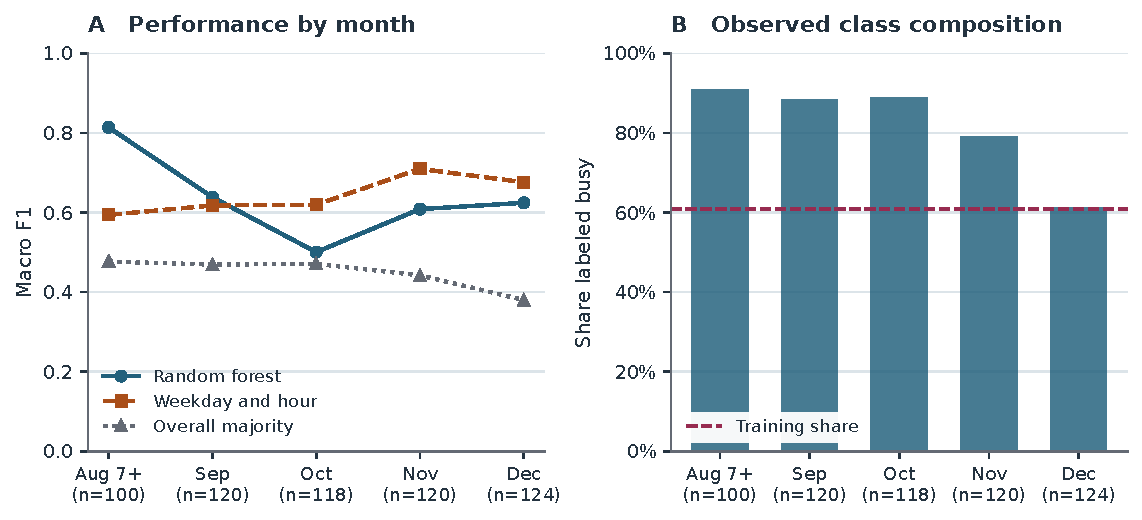
\includegraphics[width=\linewidth]{bike_monthly.pdf}
\caption{保留期間の月別内訳。左はmacro F1、右は正解ラベルの「混雑」の割合。8月は7日以降。いずれも同じ学習済みモデルと固定したルールに対する記述的な集計で、区間推定は含まない。}
\label{fig:bike}
\end{figure}

図\ref{fig:bike}のとおり、モデルは8・9月、曜日・時間帯のルールは10--12月でmacro F1が高かった。例えば8月は0.814と0.594、10月は0.500と0.619である。混雑の割合も8月91.0\%から12月61.3\%まで変化した。この観察から、後続期間全体の集計と、月別のクラス構成と結果を併記する意義が分かる。変化の原因と時系列の依存を考慮した差の区間は、本実験からは確定できない\cite{audit,milestone}。
